\chapter{Results and Discussion}
\label{chap:Results_and_Discussion}

This chapter will be divided in three parts: in the first one, the settings and parameters to perform the tests will be presented, together with the achieved results. In the second part, an analysis of these results will be developed and the third part will be a final summary.

\section{Settings and Parameters}

Since the quadrotor has only four actuators to move in six degrees of freedom, it is an underactuated system. Hence, there will be only four variables that will be controllable. The choice made was to control the $x, y, z$ positions and the orientation around the $z$ axis ($\psi$). It is important to mention that the MPC is not sending directly the input signals going to the motors. The reason for this is that the model that is being used to perform the calculations is a linearized model, therefore the state variables represent deviations around an operation point. The MPC is instead controlling these linearized state variables and sending that to modify the initial operation point. The operation point being used is calculated by simple force balance in the hover condition, to obtain the required angular speed of the rotors to keep the quadrotor static in the air, which is approximately $360$ radians per second. That way, the control signal vector going to the quadrotor simulator is built as follows:

\begin{equation*}
\mathbf{u} = \underbrace{\mathbf{\bar{u}}}_\textrm{operation point} + \underbrace{\Delta \mathbf{u}}_\textrm{controlled by MPC}
\end{equation*}

In order to adjust to this, the constraints in the input were also modified, through a displacement of the operation range for this variation of the angular speed. The original operation range is taken from the experiments realized by Sun \cite{ref:YueSun2012}, which is $130 \leq \omega_{i} \leq 500$, in radians per second. In order to be congruent with that range, the variation of the angular speed is limited between $-230 \leq \Delta \omega_{i} \leq 140$ around the operation point, again in radians per second.\\ 

Regarding the tuning of MPC, the parameters available to adjust are the horizons and the weight matrices in the cost function. The selection of a proper prediction horizon for any MPC application is dependant on the dynamics of the system that is being controlled.  This choice is of great influence in the size of the optimization problem to solve, and therefore in the computational power required to provide deterministic operation. If the horizon is too short, the prediction won't give information about future control signals and might create unstability in the controller \cite{ref:Gabrielsson2012}. On the other hand, if the horizon is too long, the optimization problem to solve could be too large to solve in each time sample. In this particular case, since the model being used for prediction is a linearized version, a very long prediction in the future might mean moving too far away from the operation point, which will cause erratic predictions due to nonlinearities. \\

With the weight matrices, the procedure is also made in a trial and error fashion. A good initial guess for the quadrotor model is taken from previous implementation parameters \cite{ref:Bouffard2012}. The simulation is performed in a computer with an Intel \textsuperscript{\textregistered} Core\texttrademark 2 Duo running at 3.0 GHz. The complete specifications for the simulation are presented in the following table.

\begin{center}
    \begin{tabular}{| l | p{7cm} |}
    \hline
    Prediction horizon & 30 samples at a frequency of 120 Hz \\ \hline
    Weight matrices & Specified in Appendix A \\ \hline
    Input constraints &  -230 \leq \Delta \omega_{i} \leq 140 [rad/s] \\ \hline
    State constraints &  -5 \leq V_x \leq 5 [m]  \newline -5 \leq V_y \leq 5 [m] \newline 0 \leq z \leq 5 [m] \\ \hline
    Processor & Intel \textsuperscript{\textregistered} Core\texttrademark 2 Duo @ 3.0 GHz
    \hline
    \end{tabular}
\end{center}

The trajectory reference used to test the MPC in the quadrotor simulator is based in simple decoupled movements in each one of the controlled directions, done one at a time. The movement consists on four stages: elevation from the floor, change in orientation (a change in the yaw angle), rotating back to the original orientation, and movements in the $X$ and $Y$ axes, in that order.\\

The results of the simulation with the mentioned parameters and settings are shown below:\\

\begin{figure}[h!]
\centering
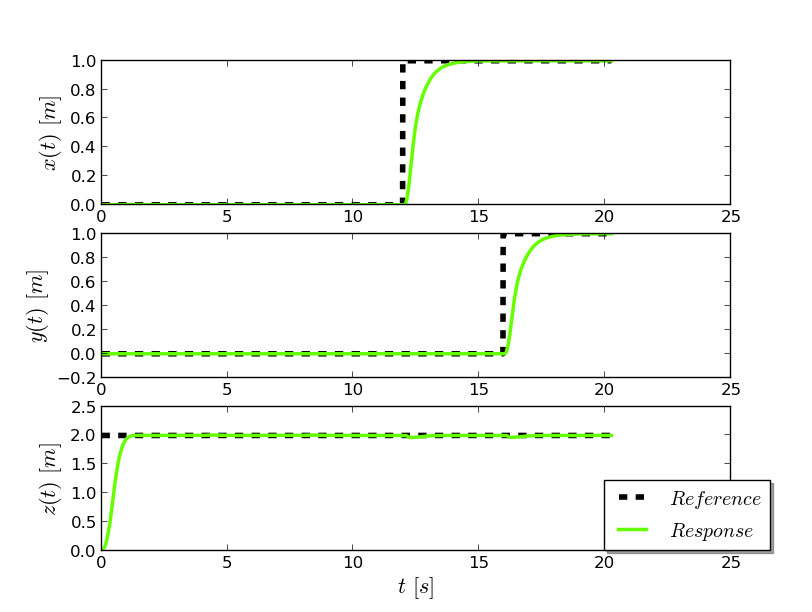
\includegraphics[scale=0.7]{Images/Chapter5/ardrone/position_control.png}
\caption{Trajectory reference and actual trajectory positions of the simulated platform.}
\label{fig:ardrone_pos}
\end{figure}

\begin{figure}[h!]
\centering
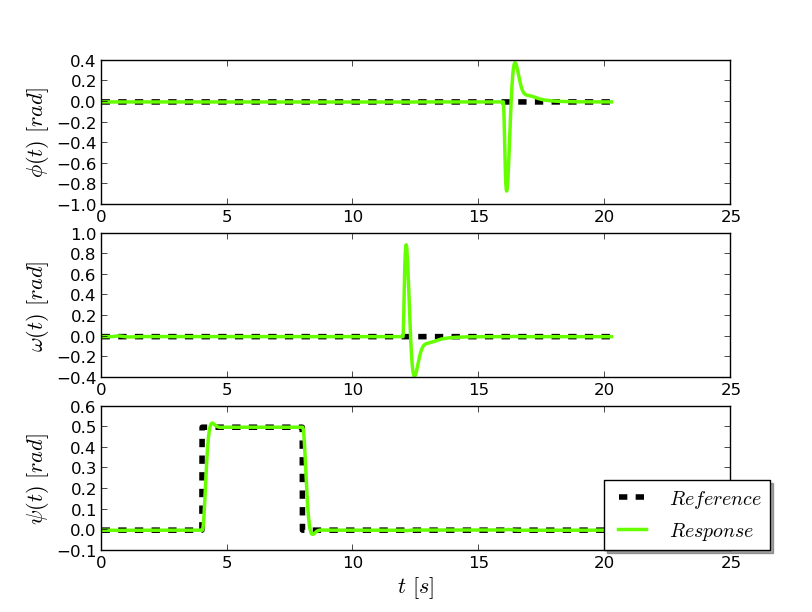
\includegraphics[scale=0.7]{Images/Chapter5/ardrone/euler_angle_control.png}
\caption{Trajectory reference and actual trajectory orientations ($\psi$) of the simulated platform.}
\label{fig:ardrone_ang}
\end{figure}

\begin{figure}[h!]
\centering
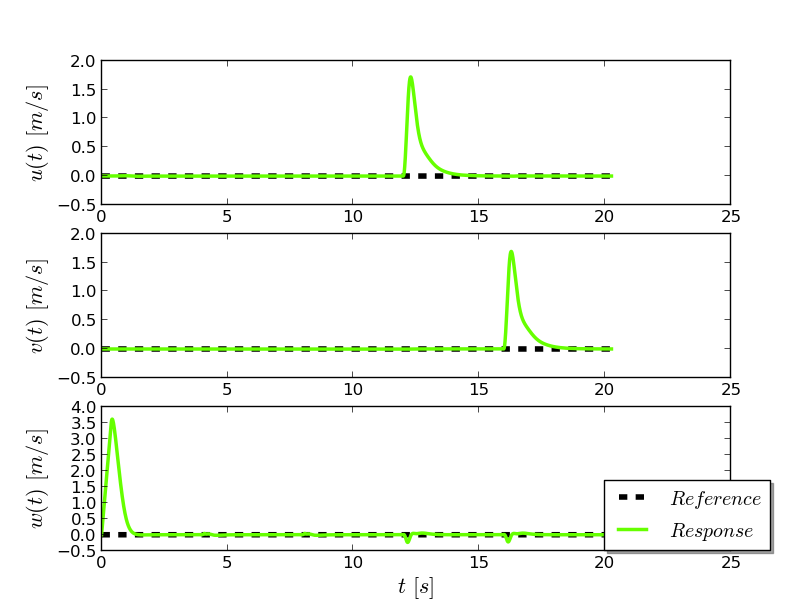
\includegraphics[scale=0.7]{Images/Chapter5/ardrone/lin_velocity_control.png}
\caption{Linear velocities of the simulated platform. }
\label{fig:ardrone_lin_vel}
\end{figure}

\begin{figure}[h!]
\centering
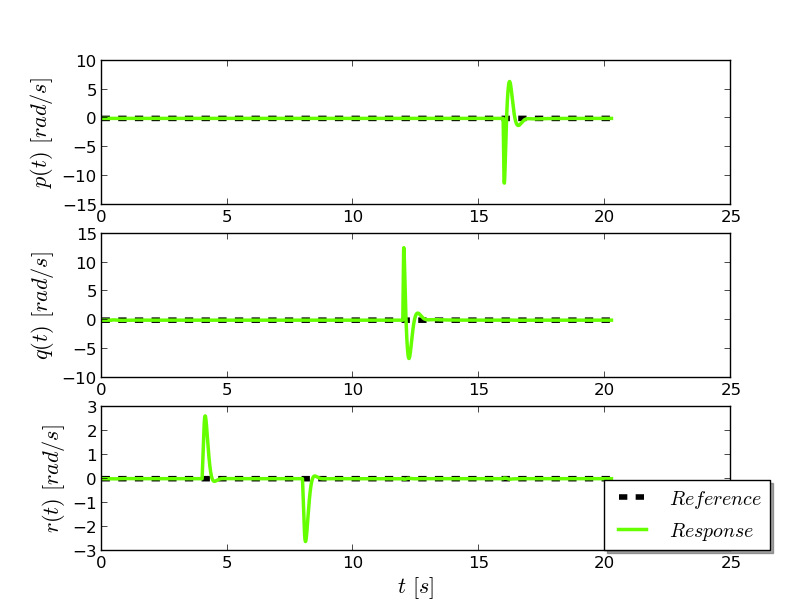
\includegraphics[scale=0.7]{Images/Chapter5/ardrone/ang_velocity_control.png}
\caption{Angular velocities of the simulated platform.}
\label{fig:ardrone_ang_vel}
\end{figure}

\begin{figure}[h!]
\centering
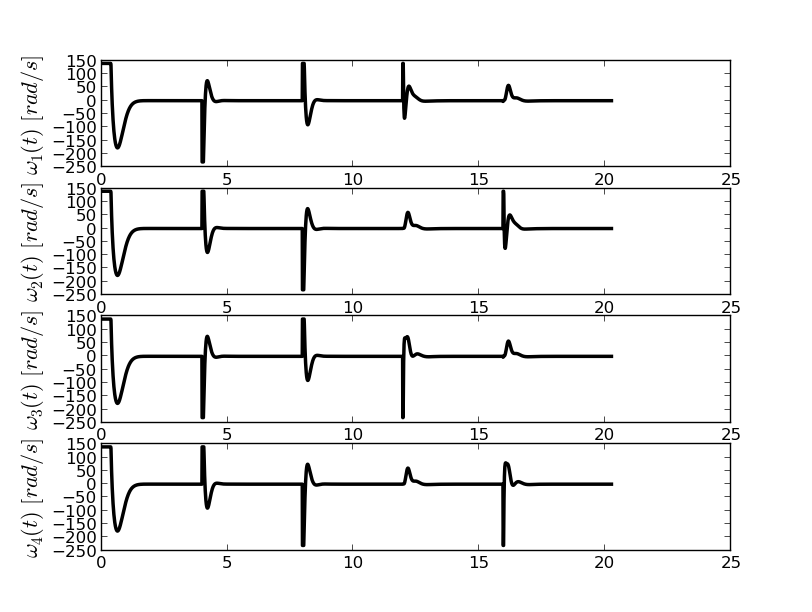
\includegraphics[scale=0.7]{Images/Chapter5/ardrone/control_signals.png}
\caption{Control signals generated by the MPC strategy.}
\label{fig:ardrone_inputs}
\end{figure}

The simulations show the performance of the MPC strategy in the simulated quadrotor. Figures \ref{fig:ardrone_pos} and \ref{fig:ardrone_ang} show the position and orientation  response of the system against step input signals on each controlled variable. The response shown presents a smooth behavior, no overshoot and a small settling time correspondant to a fast system like the quadrotor. The prediction horizon used, $N_p = 30$, has a right balance in speed to allow a fast response without overshoot.\\

The initial set of restrictions considered was bigger than the one used in the simulations shown, since there were restrictions considered on the roll and pitch angles ($\phi$ and $\theta$) taken in order to assure the stability of the quadrotor. Normally, this would be addressed by a hovering PI control loop in the original AR-Drone control architecture. However, the consideration of the constraints on these angles lead to unfeasibility in the quadratic programming problem, so  these restrictions were relaxed, and eventually dropped. The stability of the platform was addressed by strenghtening the restrictions on the velocities in the $x$ and $y$ axes, since these velocities are dependant on the roll and pitch angles. \\

The actual version of the library does not include functions to cope with unfeasibility. This must be considered in further stages of development in order to provide a better operation under the presence of more constraints. Some suggested strategies to cope with unfeasibility are referred by Camacho and Bordons \cite{ref:CamachoBordons}: an initial strategy consists of dropping the state constraints at the initial portion of the horizon in order to make the problem feasible; another way is to create soft constraints from the hard constraints stated initially, and then adding a term in the cost function to penalize constraint violation. Feasibility is important to assure closed-loop stability. One could also use the solution of the unconstrained problem  when unfeasibility appears, but this will not guarantee stability.\\

This simulation is not performed in real-time, therefore the 



